\section{Review}
\label{sec:review}

Due to recent advances in web technologies (\eg{}, WebGL and HTML5), web-based visualizations have become increasingly prevalent~\autocite{Evans.2014.CGJourn.Survey}.
%
Applications include: data visualization, education (\eg{}, viewing the human anatomy or the structure of a molecule), content creation (\ie{}, creating 3D models and other assets), gaming, and structure visualization (\eg{}, geospatial and architectural)~\autocite{Moore.2014.ALIFE.Web,Evans.2014.CGJourn.Survey,Mwalongo.2016.CompGraphForum.Web}.
%
The convenience of web-browsers and their increased performance has led to this increase in web-based applications.


\subsection{Usage}

Before we discuss Review in detail, we provide the following proposed usage for using Review as part of an ER study:

\begin{enumerate}
  \item Run evolutionary experiments
  \item Generate animation data (in Review log file format) for \emph{interesting} results
  \item Load animations in Review
  \item Configure the scene (change materials and environment)
  \item Export animation file (Review log file and/or glTF formats)
  \item (optional) Generate high-quality videos using glTF
  \item Share animations with other researchers
\end{enumerate}

The final step above can be achieved in several ways. First, Review log files can be directly sent to collaborators (e.g., via email). A log file saved on a local computer can be opened by Review through a file browser or by dropping the file onto the browser window.
%
Alternatively, log files can be hosted on any server and automatically fetched by Review in the following manner: https://review.github.io/?log=https:// raw.githubusercontent.com/review/review.github.io/master/ examples/simple-sphere.json.
%
Here, we have provided the URI of a log file to Review via an HTTP URI query component (note the "?" after the domain and the key-value pair that follows).
%
When embedding links to an animation inside of a research article, it can often be desirable to shorten the URI with a URL shortener (such as Bitly\footnote{\url{https://bitly.com/}} and Ow.ly\footnote{\url{http://ow.ly/}}) .
%
For example, this shortened link can be used in place of the previous link: \url{http://bit.ly/2HOZQcY} (this usage is also shown in the caption of Figures~\ref{fig:quad_gaits} and~\ref{fig:worm_gaits}).
%
Additionally, a QR code can be generated for the URL and paired with the image sequence as shown in Figures~\ref{fig:quad_gaits} and~\ref{fig:worm_gaits}. This will enable readers to print a copy of an article and view the animation on their smart-phone using a QR code reader.
%
% This can be useful if someone is reading a printed copy of the study in question, but they are able to visit the Review link on their smart-phone.
%
Finally, Review-based animations can be embedded into any website using an HTML \textbf{iframe}.
%
This allows users to see animations in a similar manner to an embedded video, but they will be able to manipulate the viewing angle, and change the color of objects in the scene.


% \begin{figure}[htb!]
%     \centering

%     \subfloat[Animation]{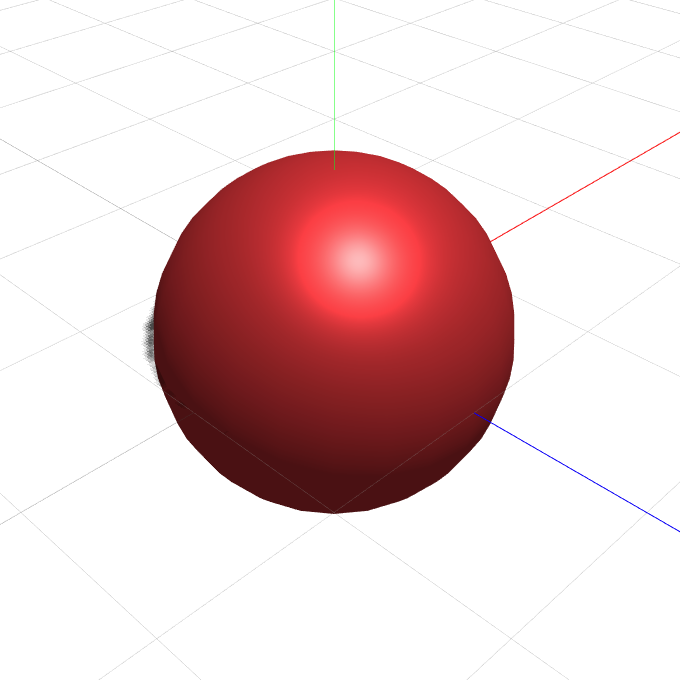
\includegraphics[width=0.25\columnwidth]{figures/sphere_ss.png}}%
%     \hfil%
%     \subfloat[QR Code]{
\includegraphics[width=0.25\columnwidth]{figures/sphere_qr.png}}

%     \caption{(a) An image of the animation and (b) a QR Code directing a reader to the animation on Review.}
%     \label{fig:sphere_qr}

% \end{figure}



\subsection{Interface}


A screen-shot of the Review interface is shown in Figure~\ref{fig:review_screenshot}.
%
Review provides two methods for loading a log file (the log files is described in the next section):
(1) log files can be loaded from the local machine either by dragging the file onto the browser window, or by choosing a file from the open-file dialog box that is available when no log file is currently loaded (not shown), or
(2) log files can be specified via an HTTP URI query component and loaded automatically by Review from remote servers (as demonstrated in the ``Usage'' section above).


\begin{figure}[htb!]
\centering
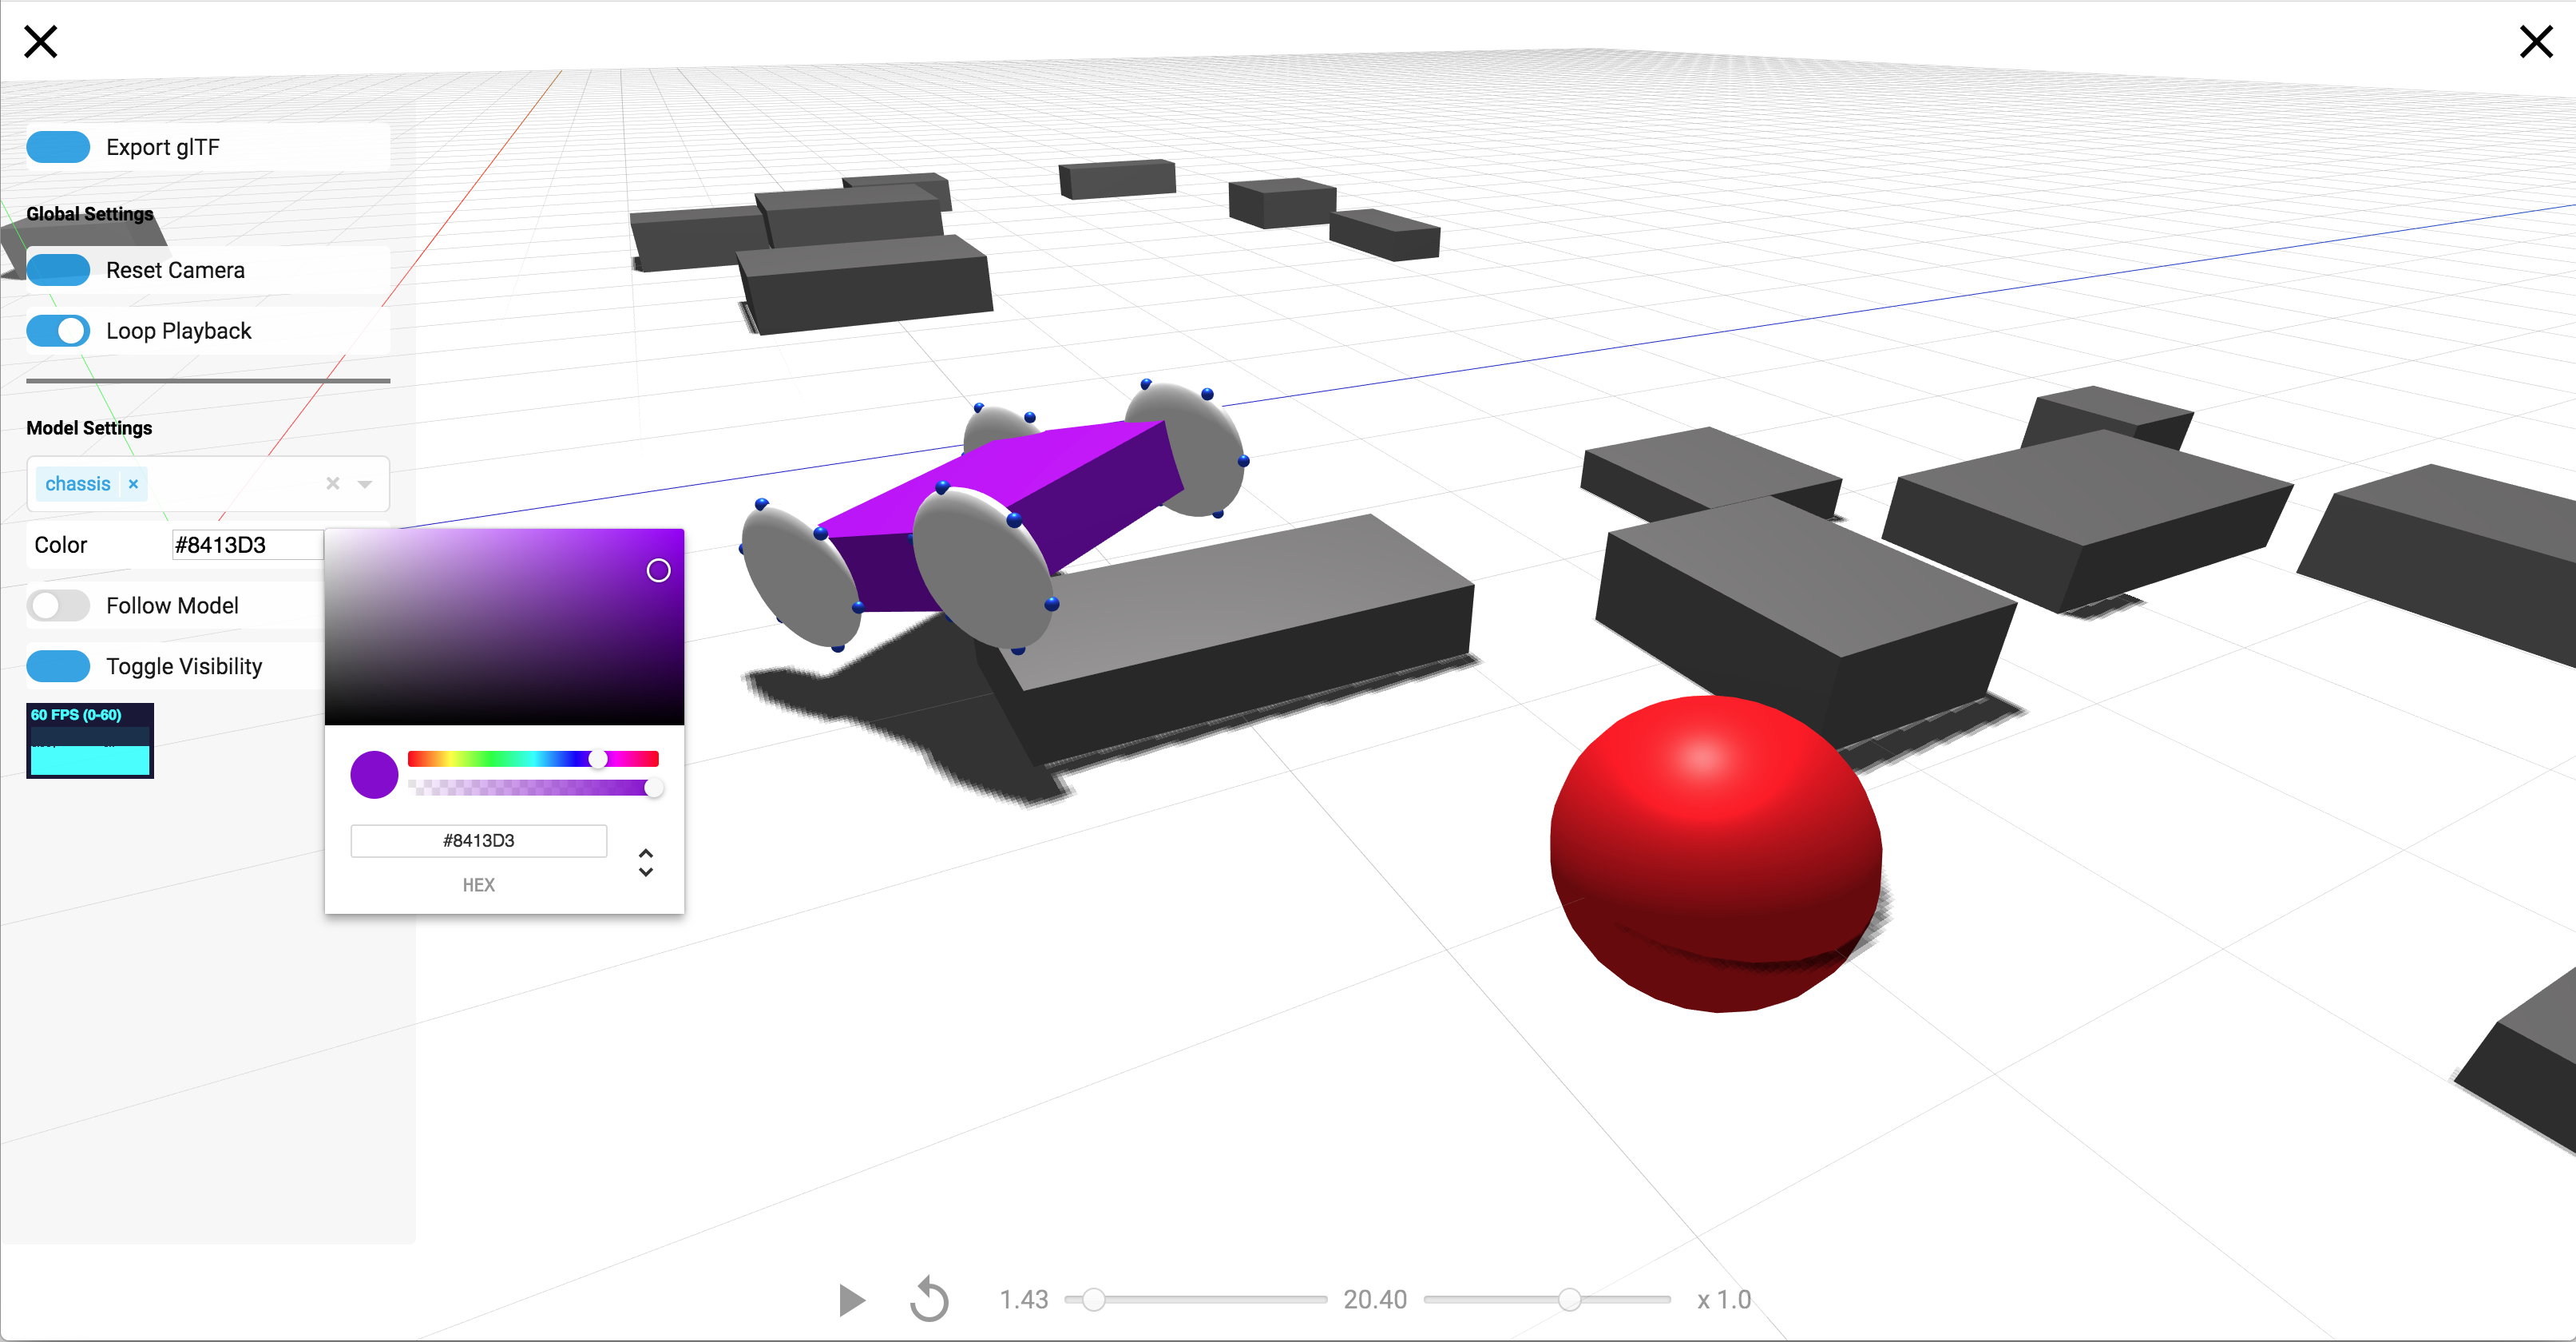
\includegraphics[width=0.9\columnwidth]{figures/review-screenshot.png}
\caption{A screen-shot of Review with a UGV simulation in progress. The color palette can be used to change the color of each object in the scene.}
\label{fig:review_screenshot}
\end{figure}


This image depicts a scene of a transformable wheel UGV and several obstacles; the UGV's chassis color is currently being changed with a color picker that can be accessed in the settings pane.
%
Review's settings pane includes several other expected features, for example, the ability to follow a specific object with the camera, reset the camera to its original settings, change the visibility of objects in the scene, and export the current animation.
%
The settings pane can be hidden from view when it is unneeded.
%
A standard set of playback controls are available at the bottom of the screen.
%
One of the most useful controls is the progress bar, which can be \emph{scrubbed} forward and backwards. Scrubbing refers to the ability to drag the progress icon to quickly navigate through time while watching the scene update on-the-fly.
%
The playback speed can be adjusted from~\numrange{-5}{5}, where a negative number indicates that the scene will play in reverse.




\subsection{Log File Format}

One motivating factor for developing Review was the lack of an alternative application with a suitable file format.
%
Most similar tools (described in section~\ref{sec:related_work}) require a complex file format that is difficult to generate alongside a physical simulation--likely because most 3D object viewers anticipate that visualization data is being generated by an authoring tool like Blender~\autocite{Blain.2012.Book.Blender} or Autodesk Maya~\autocite{Palamar.2015.Book.Maya}.
%
Common 3D file formats that include animations (\eg{}, COLLADA, FBX, glTF, and OpenGEX) focus on making it easy to load binary data and immediately send it through a GPU-centric graphics pipeline.
%
For example, the following components are needed to specify a moving sphere in the glTF file format:


\begin{enumerate}

  \item A binary data buffer specifying the 3 dimensional positions of all points comprising the sphere, the surface normals of all points, and texture coordinates;

  \item A set of buffer accessors (called ``views'') for specifying how to extract positions, normals, and texture coordinates from the binary buffer;

  \item A material object that specifies various properties of the sphere's surface (\ie{}, roughness, metallic factor, and base color);

  \item A mesh object that groups together the buffer accessors associated with a single object and includes a reference to the sphere's material;

  \item A node object that refers to the above mesh and specifies the sphere's relationship to all other objects in the scene (even if no other objects are present);

  \item A scene graph specifying that the sphere is a root object (it's transform does not depend on any other objects);

  \item An animation object that specifies how the sphere is transformed (typically translations, rotation, and scale) over time.

\end{enumerate}


glTF version 2.0 was released in 2017 and is a relatively simple specification compared to the other formats listed above.
%
In contrast, the Review file format was specifically designed to be easily generated while running a simulation. An example of the Review log file format is provided in Listing~\ref{lst:logfile}.
%
This is a visualization of a sphere that moves in a square pattern and pauses for one frame when it reaches its position defined in the fourth frame.
%
This example animation can be viewed at the following link: \url{http://bit.ly/2HOZQcY}.


\begin{minipage}{\linewidth}
\begin{lstlisting}[style=json, caption={Review Log File Example}, label=lst:logfile]
{
  "name": "Sphere Example",
  "timeStep": 0.25,
  "objects": [{
    "name": "sphere1",
    "mesh": "sphere"
  }],
  "frames": [
    { "sphere1": { "t": [0, 0, 0] } },
    { "sphere1": { "t": [1, 0, 0] } },
    { "sphere1": { "t": [1, 0, 1] } },
    { "sphere1": { "t": [0, 0, 1] } },
    {  },
    { "sphere1": { "t": [0, 0, 0] } }
  ]
}
\end{lstlisting}
\end{minipage}


The log file is a JSON file with a specific schema~\autocite{JSON.2018.Schema}. Here we describe a basic file, but the full schema can be found in the Review Git repository.
%
This file format is human readable and writable, and nearly all programming languages include a library for manipulating JSON data.
%
The Review logging library\footnote{\url{https://github.com/review/logger-cpp}} used to generate the  files linked in this study has been provided, and it contains less than 100 lines of C++ code and has only one external dependency (a C++ JSON library).
%
This format has four required fields. The \textbf{name} (string) and \textbf{timeStep} (number) provide a unique name for the visualization and the time elapsed between frames, respectively.


\textbf{objects} (array) is a list of all objects that are present in the scene. In the example, there is only one object and only the required object fields are specified.
%
Each object must have a unique \textbf{name} (string) and a \textbf{mesh} (string).
%
The \textbf{mesh} value denotes either a primitive (\emph{cube}, \emph{cylinder}, or \emph{sphere}) or a URI to an external resource (\eg{}, an STL or COLLADA file).
%
In addition to these fields, several other attributes can be specified. The most prominent fields include: a physically based rendering (PBR) material, translation, rotation, and scale.


\textbf{frames} (array) is a list of all frames in the scene. The time lapsed between each pair of consecutive frames is always \textbf{timeStep}.
%
Each frame is a JSON object where the keys (left side of the colon) denote objects named in the \textbf{objects} array, and the values (right side of the colon) denote object transformations.
%
In the example, the only attribute of \emph{sphere1} that changes is its translation. The most common animation attributes are translation (\textbf{t}) and rotation (\textbf{r}), but other types can be specified (\eg{}, scale).
%
As exemplified by the fifth frame, this log file format allows for empty frames. An empty frame signifies that no objects are in motion during that frames time step. Allowing for empty frames greatly reduces the file size when many objects are in a given scene but only a few are in motion at a specific time.
%
For example, for the UGV visualization in Figure~\ref{fig:review_screenshot} all 30 boxes are dynamic, but only one or two boxes are pushed by the UGV in any given frame.
%
Although frame data may be omitted, currently the empty frames themselves must be present to ensure that the duration of the simulation is accurate--the log file format does not currently allow for variable \textbf{timeSteps} between different frames.






\subsection{Technical Details}

After Review loads a JSON-format log file, it converts it into glTF~2.0\footnote{\url{https://github.com/KhronosGroup/glTF}}.
%
glTF is a transmission format specified in JSON that is used for loading and saving 3D models and scenes--an example of the contents of a glTF file are described above.
%
It is advantageous to convert the Review log file into a format that is readily loaded by graphics engines.
%
A custom graphics engine could be constructed around the Review log format (indeed, an earlier version of Review used a custom engine), however it is beneficial to use a full-featured graphics engine with state-of-the-art features and optimizations.
%
We chose glTF due to its wide support and relatively simple specification.
%
% In our early implementations of Review, we were using the Review log files directly, however, by converting to glTF we can rely on well-tested and optimized animation frameworks for visualizing robot behaviors.
%
Thus, Review maintains the benefit of a simple file format while also gaining the capabilities of more capable rendering libraries.


Review uses three.js~\autocite{Cabello.2013.ThreeJS} to render animated scenes to a browser window.
%
three.js includes a modern rendering pipeline built on WebGL~\autocite{WebGL.2018}, great support for animations, and the ability to import glTF files.
%
WebGL is a JavaScript API for rendering 3D graphics within a browser. WebGL enables GPU accelerated rendering in a similar fashion to OpenGL (specifically OpenGL ES). GPU shaders can be customized to produce stunning visuals that are rendered in the browser in real-time.
%
WebGL is supported on many systems, including most modern desktop browsers and many browsers running on iOS and Android.


three.js is a cross-browser JavaScript library created to make 3D graphics applications.
%
It includes many features for building complex scenes from simple components: different forms of lighting, different material and texture models, support for importing standard mesh formats, and an animation system.
%
Perhaps the most important feature of the three.js animation system is \emph{interpolation}, whereby three.js will interpolate transformation between frames.
%
In the moving sphere example above, the time between frames is 0.25s, however, most computers will have no trouble rendering the scene at 60 frames-per-second, which means that three.js will use interpolation to generate roughly 15 frames in-between each frame.
%
The impact of interpolation is most dramatic when the playback speed is reduced. For instance, when the playback speed is set to 0.25 three.js generates 60 interpolated frames, thereby providing a smooth animation.
%
Without interpolation, animations would be choppy (similar to a slowed-down video).
